\documentclass{beamer}

\usetheme{Berkeley}

\begin{document}
\title{SDMdata}
\subtitle{A GBIF data collect tools}
\author{Xiaoquan Kong}
\institute[]{}
\subject{}
\keywords{}
\logo{
\includegraphics[height=0.8cm]{image/logo.png}}
\date{2014-8-18}

\maketitle
\section{Introduce}
\begin{frame}
	\frametitle{Introduce}
	\framesubtitle{What is SDMdata}
	\begin{itemize}
		\item SDMdata is a web-based tools to help species distribution researcher to more efficiency collect species occurrence data.
		\item It brings some automatic function to help user find potential error.
		\item Yes, it's open source software (AGPL licensed). 
	\end{itemize}
\end{frame}
\begin{frame}
    \frametitle{Introduce}
    \framesubtitle{Advantage of SDMdata}
    \begin{itemize}
	    \item Automatic check species name compare with GBIF
	    \item Web-based interface allow you access from everywhere
	    \item Optional cross check to automatic mark potential occurrence point
    \end{itemize}
\end{frame}
\section{Usage}
\begin{frame}
	\frametitle{How to use SDMdata}
	\framesubtitle{Workflow}
	\begin{enumerate}
		\item Import species name
		\item Check species name \(automaticly\).
		\item Collect species occurrence record
		\item Cross check species occurrence point
		\item Export data
	\end{enumerate}
\end{frame}
\section{Demonstrate}
\begin{frame}
	\frametitle{Login}
	\framesubtitle{Login and default admin}
	\begin{center}
		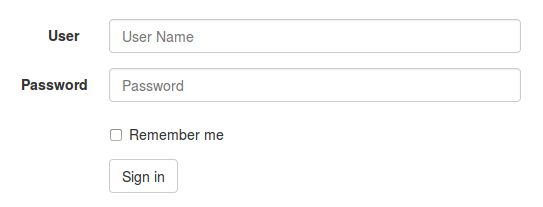
\includegraphics[scale=0.3]{image/login.png}
	\end{center}
	Software build-in administrator account: admin
	\newline Admin initial password: admin
\end{frame}
\begin{frame}
	\frametitle{Import species name}
	\framesubtitle{Main ectrance}
	This is main entrance point of import species name:
	\begin{center}
		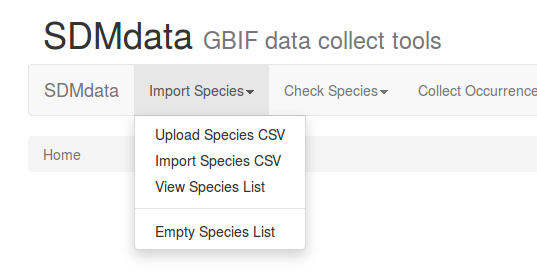
\includegraphics[scale=0.3]{image/import_species.png}
	\end{center}

\end{frame}
\begin{frame}
	\frametitle{Import species name}
	\framesubtitle{Upload CSV file}
	Upload a CSV file that contain species name 
	\begin{center}
		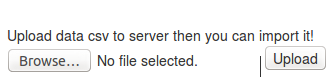
\includegraphics[scale=0.5]{image/upload_csv.png}
	\end{center}

\end{frame}
\begin{frame}
	Here is a example of csv file:
	\begin{center}
		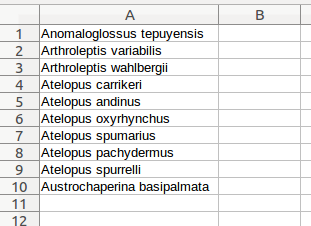
\includegraphics[scale=0.5]{image/csv_example.png}
	\end{center}
	\begin{block}{Notice}
		CSV file MUST encode in ASCII, and first column MUST be species name
	\end{block}
\end{frame}
\begin{frame}
	Import CSV file into software:
	\begin{center}
		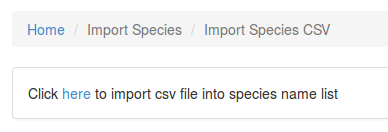
\includegraphics[scale=0.5]{image/import_csv.png}
	\end{center}
\end{frame}
\begin{frame}
	View imported species name:
	\begin{center}
		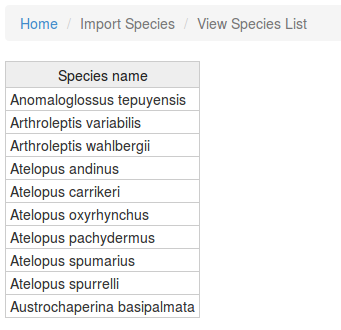
\includegraphics[scale=0.5]{image/view_species_name.png}
	\end{center}
\end{frame}
\begin{frame}
	This is main entrance point of check species name:
	\begin{center}
		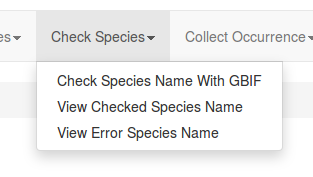
\includegraphics[scale=0.5]{image/check_species_all.png}
	\end{center}
\end{frame}
\begin{frame}
	The control page of check species name:
	\begin{center}
		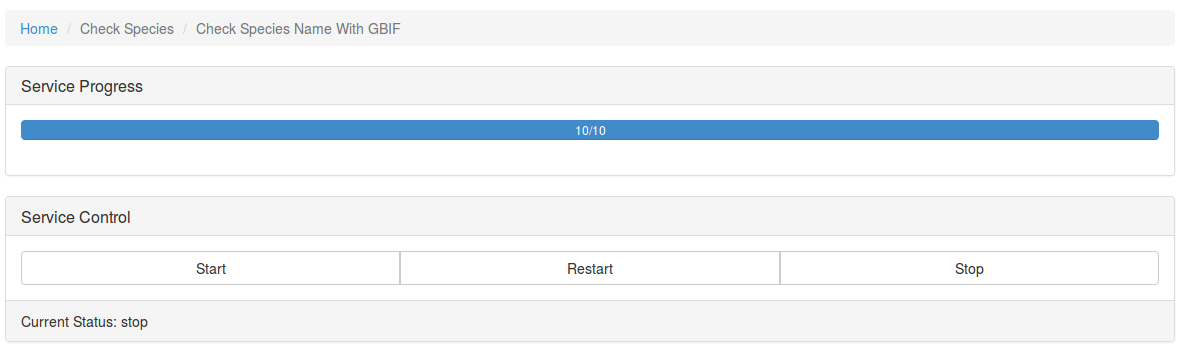
\includegraphics[scale=0.2]{image/control_check_species.png}
	\end{center}
\end{frame}
\begin{frame}
	View checked species name:
	\begin{center}
		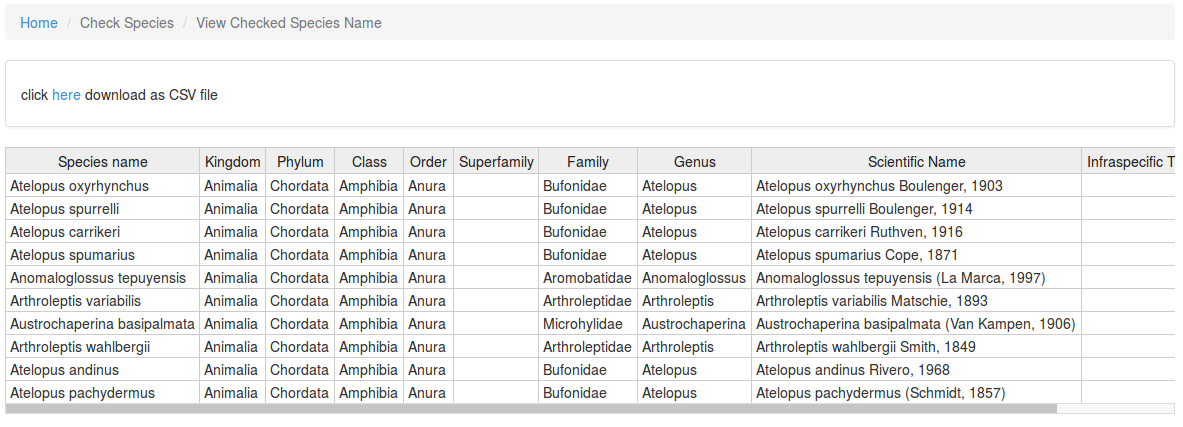
\includegraphics[scale=0.2]{image/checked_species_name.png}
	\end{center}
\end{frame}
\begin{frame}
	Control fetch occurrence:
	\begin{center}
		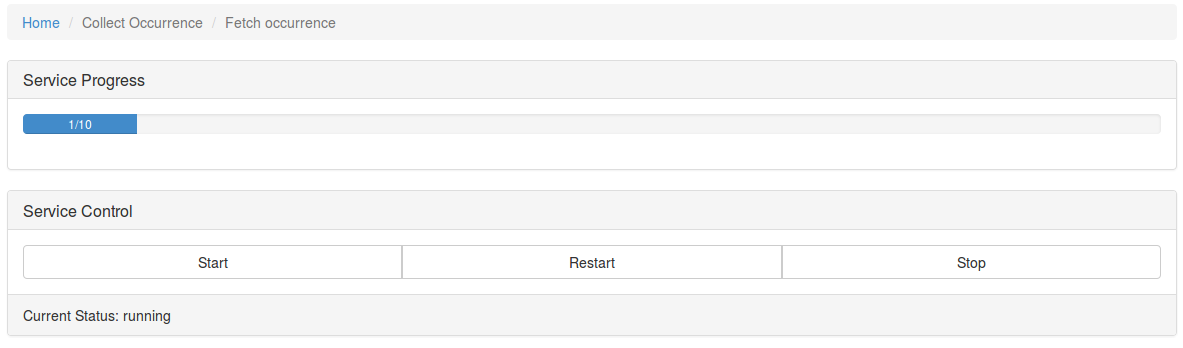
\includegraphics[scale=0.2]{image/control_collect_occurrence.png}
	\end{center}
\end{frame}
\begin{frame}
	\frametitle{Cross check}
	\framesubtitle{Why?}
	Species occurrence data come fro GBIF always contains some errors, it cannot be used directly.
	\newline After some data clean jobs, that will remove errors. Cross check is one of many clean method.  
\end{frame}
\begin{frame}
	\frametitle{Cross check}
	\framesubtitle{How?}
	GBIF occurrence data with coordinate always come with country which the point belong to.
	Our cross check will check the coordinate with country, to check if it match.
	If not match that means this occurrence record \textbf{may} have some mistake.  
\end{frame}
\begin{frame}
	Control cross check:
	\begin{center}
		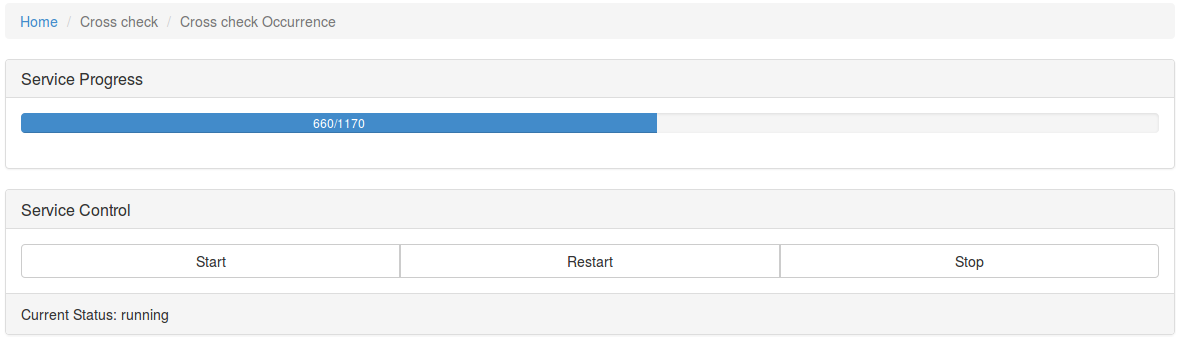
\includegraphics[scale=0.2]{image/control_cross_check.png}
	\end{center}
\end{frame}
\begin{frame}
	View cross check result:
	\begin{center}
		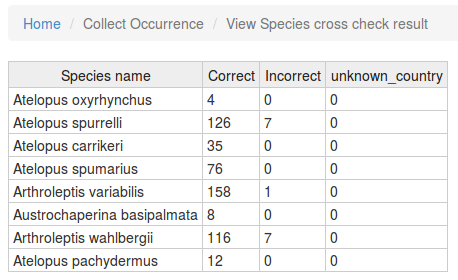
\includegraphics[scale=0.4]{image/view_cross_check.png}
	\end{center}
\end{frame}
\begin{frame}
	Export species occurrence data:
	\begin{center}
		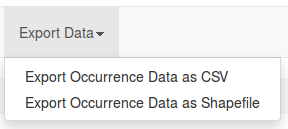
\includegraphics[scale=0.4]{image/export_data.png}
	\end{center}
\end{frame}
\begin{frame}
	Directory of species occurrence data:
	\begin{center}
		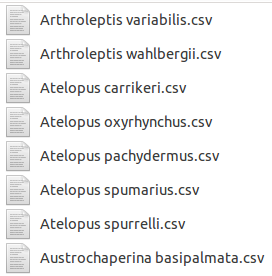
\includegraphics[scale=0.4]{image/data_dir.png}
	\end{center}
	Each species have a CSV file named with the species name.
\end{frame}
\begin{frame}
	CSV file of each species occurrence data:
	\begin{center}
		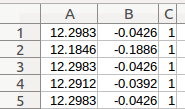
\includegraphics[scale=0.4]{image/csv_structure.png}
	\end{center}
	Each row represent a occurrence point
	\newline First column is longitude, second column is latitude, third is the cross check code, check code have different value:
	\begin{itemize}
		\item 1: means cross check is pass
		\item 0: means cross check is failed, that indicate this occurrence point have potential issue.
		\item -1: means this occurrence point provide a unknown country code
	\end{itemize}
\end{frame}
\end{document}
